\documentclass[a4]{article}

\usepackage[left=3cm,right=3cm,top=2cm,bottom=2cm]{geometry} 

\usepackage[utf8]{inputenc}   % otra alternativa para los caracteres acentuados y la "ñ"
\usepackage[           spanish % para poder usar el español
                      ,es-tabla % para los captions de las tablas
                       ]{babel}   
\decimalpoint %para usar el punto decimal en vez de coma para los números con decimales

\usepackage[bookmarks=true,
            bookmarksnumbered=false, % true means bookmarks in 
                                     % left window are numbered              
            bookmarksopen=false,     % true means only level 1
                                     % are displayed.
            colorlinks=true,
            linkcolor=blue,
            urlcolor=cyan]{hyperref}
            
\usepackage[T1]{fontenc}
\usepackage{lmodern}

\usepackage{parskip}
\usepackage{xcolor}

\usepackage{caption}

\usepackage{listings}
\lstset
{ %Formatting for code in appendix
    language=C++,
    basicstyle=\footnotesize,
    numbers=left,
    stepnumber=1,
    showstringspaces=false,
    tabsize=1,
    breaklines=true,
    breakatwhitespace=false,
}

\usepackage{enumerate}% paquete para poder personalizar fácilmente la apariencia de las listas enumerativas

\usepackage{graphicx} % figuras
\usepackage{subfigure} % subfiguras

\definecolor{gris}{RGB}{220,220,220}
	
\usepackage{float} % para controlar la situación de los entornos flotantes

\restylefloat{figure}
\restylefloat{table} 

\newcommand{\HRule}{\rule{\linewidth}{0.5mm}}

\author{David Cabezas Berrido}
\date{\vspace{-5mm}}

\title{\huge Práctica 2: Algoritmos Divide y Vencerás \HRule\vspace{-4mm}}

\setcounter{section}{-1}

\begin{document}
\maketitle
\vspace{20mm}
\tableofcontents
\newpage

\section{Problema}
Dado un vector de enteros $v$ ordenado de forma no decreciente, se
pide determinar si existe un índice $i$ cumpliendo
$v[i]==i$. Trataremos dos casos, con todos los elementos del vector
diferentes y admitiendo elementos repetidos.

\section{Algoritmo ``obvio''}
En cualquiera de los casos, la solución más sencilla del algoritmo es
recorrer el vector desde un extremo hasta que se llega al final o se
encuentra el índice $i$ que buscamos. Claramente su eficiencia teórica
es lineal. Se visualizará su eficiencia empírica en cada caso.

\section{Primer caso: Todos los elementos son diferentes}
En este caso, he ideado un algoritmo similar al de búsqueda binaria.

\begin{lstlisting}
  int enSuPosicion(int *T, int n){
  
  int result = -1;
  int left=0, right=n-1;
  int p = (left+right)/2;
  bool found = false;
  
  while(!found and left <= right){
    if(p == T[p]){
      result = p;
      found = true;
    }
    else if(p < T[p])
      right = p-1;
    else
      left = p+1;

    p = (left+right)/2;
  }

  return result;
}
\end{lstlisting}

Elegimos la posición del medio entre la izquierda y la derecha.  Si
el índice escogido cumple la condición, lo devolvemos. Si el valor
de la componente es mayor que el índice, podemos desechar la mitad
derecha del vector, puesto que como $p < T[p] < T[p+1]$, entonces se
tiene por ser números naturales que $p+1 \leq T[p] < T[p+1]$, por
tanto $p+1$ no cumpliría la condición y por el mismo razonamiento
ninguno de los índices mayores lo haría. Razonando de forma análoga,
si $p > T[p]$, podemos desechar la mitad izquierda del vector.

Repetimos el proceso sobre el vector restante hasta encontrar un
índice $p$ que cumpla la condición o hasta desechar todos los
elementos. Como en cada iteración desechamos la mitad del vector, el
número de iteraciones son (en el peor caso) el número de veces que
podemos dividir el número de elementos del vector en dos, es decir
$\log_2n$. Como la eficiencia de cada iteración es constante, la
eficiencia teórica del algoritmo es $O(\log n)$. Bastante más
eficiente que el algoritmo ``obvio'', que es $O(n)$.

En la figura \ref{fig:comp-distintos} se aprecia que el tiempo de
ejecución de este algoritmo es mucho más bajo que el del ``obvio''.
Mientras que las gráficas de la figura \ref{fig:ajust-distintos}
confirman la eficiencia teórica de cada uno de ellos.

\begin{figure}[H]
  \centering
  \caption{Algoritmo DyV frente al ``Obvio'' en el caso de elementos distintos.}
  \label{fig:comp-distintos}
  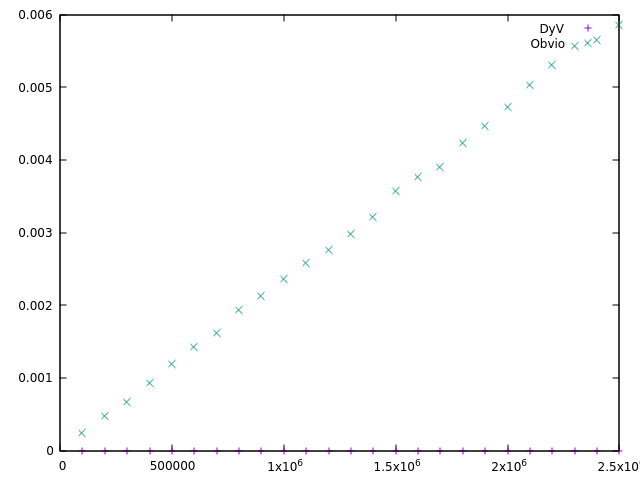
\includegraphics[width=100mm]{graficos/comparacion}
\end{figure}

\begin{figure}[H]
  \centering
  \caption{Ajuste de ambos algoritmos en el caso de elementos distintos.}
  \label{fig:ajust-distintos}
  \subfigure[Ajuste del algoritmo
  ``Obvio'']{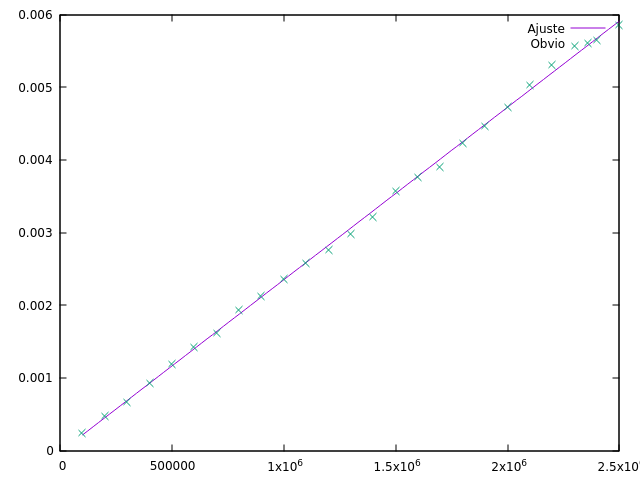
\includegraphics[width=70mm]{graficos/ajusteObvio}}
  \subfigure[Ajuste del algoritmo
  DyV]{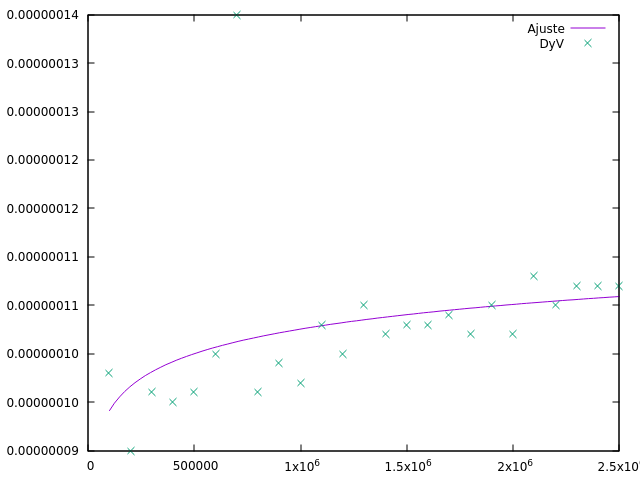
\includegraphics[width=70mm]{graficos/ajusteDyV}}
\end{figure}

Para ajustar los tiempos del algoritmo ``obvio'', he usado la función
\\ $f(x)=2.37482\mbox{e}-09x-2.47917\mbox{e}-05$. Para el ajuste del
algoritmo Divide y Vencerás, la función
$g(x)=3.66877\mbox{e}-09\log(0.975496x+1)+5.19407\mbox{e}-08$.

\section{Se repiten elementos}
El razonamiento anterior no es válido cuando el vector tenga elementos
repetidos, de hecho no es difícil encontrar ejemplos en los que el
algoritmo falle. Por ejemplo si consultamos la posición 30 y
encontramos el valor 50, no podemos descartar la parte derecha del
vector ya que este podría tener el valor 50 en todas las posiciones
desde la 30 hasta la 50, y el índice 50 cumpliría la condición.

Pero podemos obtener algo de información, puesto que en este caso
podríamos asegurar que ningún índice entre el 30 y el 49 cumplirá la
condición. Basándome en este razonamiento, he elaborado un algoritmo
para este caso. Similar al anterior, pero en vez de descartar la mitad
del vector, descarta sólo la parte en la que puedo asegurar que no hay
un índice que cumpla la condición. El algoritmo es una función
recursiva y trato los dos trozos de vector que quedan por separado.

Basta llamarlo con los límites 0 y $n$.

\begin{lstlisting}
int enSuPosicionLims(int *T, int l, int r){

  if(r <= l)
    return -1;
  
  int p = (l+r-1)/2;
  
  if(p == T[p])
    return p;

  int res;
    
  if(p < T[p]){
    if((res = enSuPosicionLims(T, l, p)) != -1)
      return res;

        
    return enSuPosicionLims(T, T[p], r);
  }
    
  if((res = enSuPosicionLims(T, p+1, r)) != -1)
    return res;
      
  return enSuPosicionLims(T, l, T[p]+1);
}
\end{lstlisting}

En el peor de los casos, sólo podemos descartar el índice que
consultamos (por ejemplo si en la posición 30 encontramos un 31), por
lo que este algoritmo tiene una eficiencia teórica de $O(n)$. Sin
embargo, en la mayoría de casos podemos descartar varios elementos del
vector en una sóla iteración. Por lo que la eficiencia empírica de
este algoritmo es mucho mejor que la del algoritmo obvio, como puede
verse en la figura \ref{fig:comp-repetidos}, de hecho, la gráfica de
este algoritmo se asemeja más a una función logarítmica que a una
líneal (figura \ref{fig:dyv-repetidos}).

\begin{figure}[H]
  \centering
  \caption{Algoritmo DyV frente al ``Obvio'' en el caso de elementos repetidos.}
  \label{fig:comp-repetidos}
  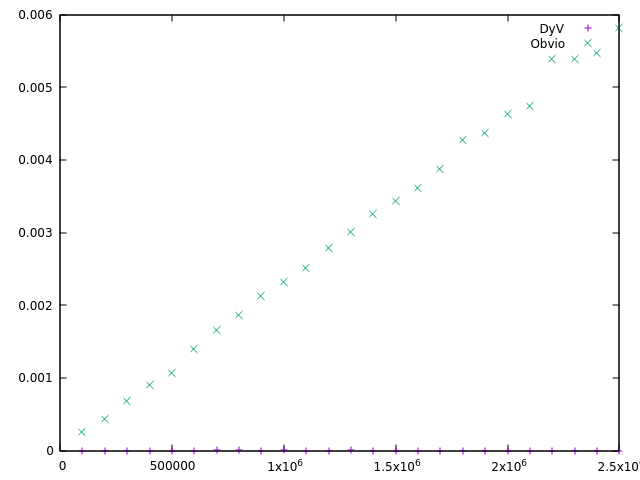
\includegraphics[width=100mm]{graficos/comparacion_Repetidos}
\end{figure}

\begin{figure}[H]
  \centering
  \caption{Algoritmo DyV para el caso de elementos distintos.}
  \label{fig:dyv-repetidos}
  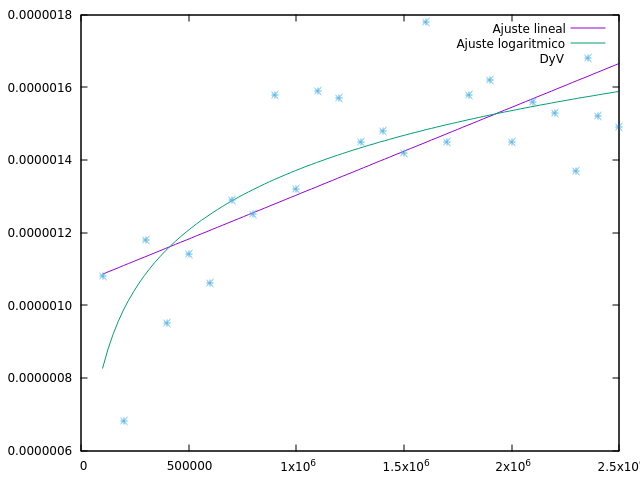
\includegraphics[width=100mm]{graficos/ajustes-rep}
\end{figure}

He ajustado los resultados con las funciones:
\[f(x) = 2.41769 \mbox{e} -13x + 1.0613 \mbox{e} -06\]
\[g(x) = 2.37005 \mbox{e} -07\log(0.975496x+1)-1.89703 \mbox{e} -06\]

Para $f$, he obtenido una RMS (Root Mean Square) de 1.77413e-07,
mientras que para $g$, la RMS ha sido de 1.61174e-07. Por tanto la
función logarítmica aproxima mejor la gráfica.

\section{¿Los ejemplos son adecuados?}
% \setcounter{subfigure}{0}

Se nos ha dado un programa que genera ejemplos con valores entre
$-n+1$ y $n-1$, donde $n$ es la capacidad del vector. Este rango de
valores provoca que los últimos índices tengan más probabilidad de
cumplir la condición que los índices más bajos. La falta de
aleatoriedad que esto provoca puede distorsionar el rendimiento del
algoritmo ``obvio''.

Lo más común es que el algoritmo ``obvio'' recorra el vector desde
el principio hasta encontrar el elemento o llegar al final. Pero es
perfectamente razonable implementar este algoritmo de forma que
recorra el vector hacia atrás, empezando desde el final. La
eficiencia teórica del algoritmo sigue siendo $O(n)$, sin embargo,
la eficiencia empírica no lo refleja nada bien, debido a que las
ejecuciones sobre vectores que cumplen la condición tienen un tiempo
muchísimo menor, ya que encuentra el elemento entre los últimos
elementos en un tiempo muchísimo menor que el que tardaría en
recorrer todo el vector.

En la figura \ref{fig:ajust-obvio-inverso}, pueden distinguirse
claramente los casos en los que el vector cumple la condición de los
que no.

\begin{figure}[H]
  \centering
  \caption{Ajuste de algoritmo ``Obvio'' empezando por el final del
    vector.}
  \label{fig:ajust-obvio-inverso}
  \subfigure[Todos los elementos son
  distintos]{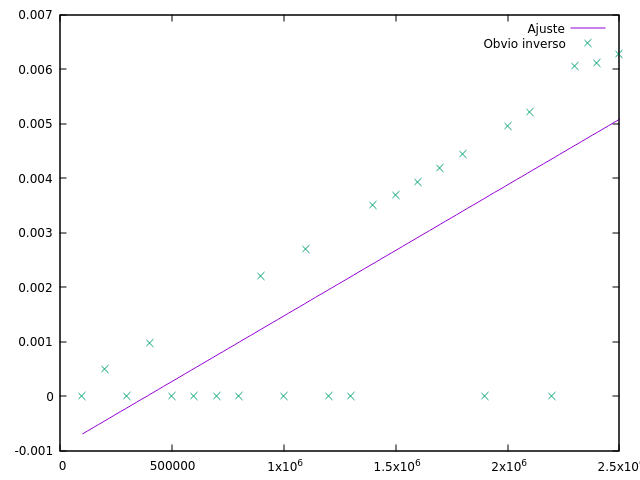
\includegraphics[width=70mm]{graficos/ajuste_obvio-inverso-distintos}}
  \subfigure[Hay elementos
  repetidos]{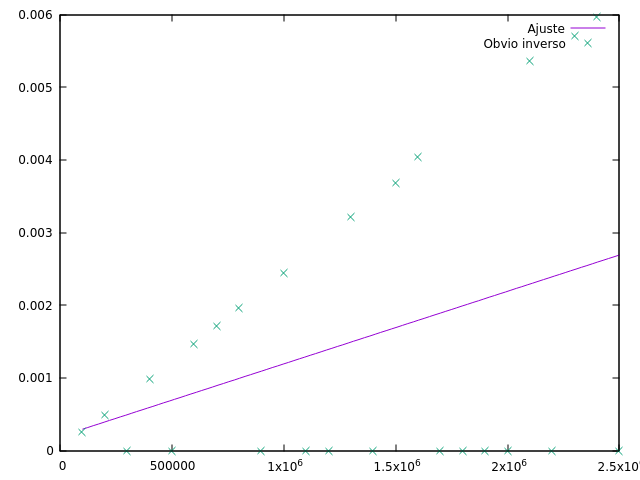
\includegraphics[width=70mm]{graficos/ajuste_obvio-inverso-repetidos}}
\end{figure}

La función de la izquierda es $f(x)=2.40612\mbox{e}-09x-0.000937639$,
y su ajuste tiene una RMS de 0.0016428. Mientras que la función de la
derecha es $g(x)=9.99324\mbox{e}-10+0.000192786$ y tiene una RMS de
0.00191864. Estos valores son mucho más altos que las RMS del resto de
ajustes, debido a que los ejemplos no son totalmente aleatorios.

Para solucionar este problema, he realizado 100 mediciones con
ejemplos diferentes, y he hecho la media de los tiempos obtenidos.
Así he obtenido datos que se ajustan mejor a la eficiencia teórica
como se observa en la figura \ref{fig:ajust-sol-obvio-inverso}

\begin{figure}[H]
  \centering
  \caption{Ajuste de algoritmo ``Obvio'' empezando por el final del
    vector.}
  \label{fig:ajust-sol-obvio-inverso}
  \subfigure[Todos los elementos son
  distintos]{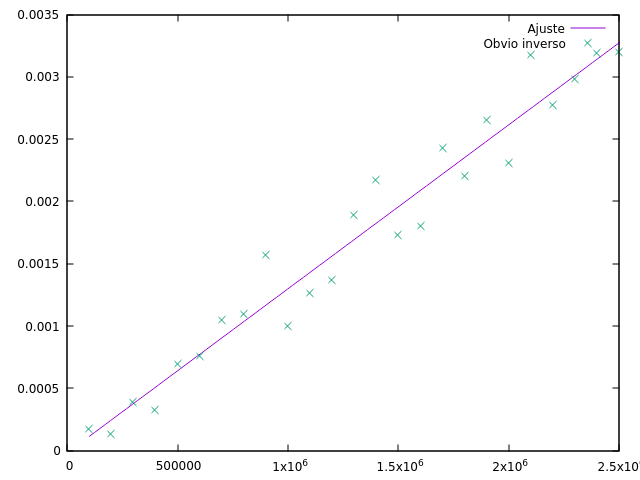
\includegraphics[width=70mm]{graficos/ajust-sol-dist}}
  \subfigure[Hay elementos
  repetidos]{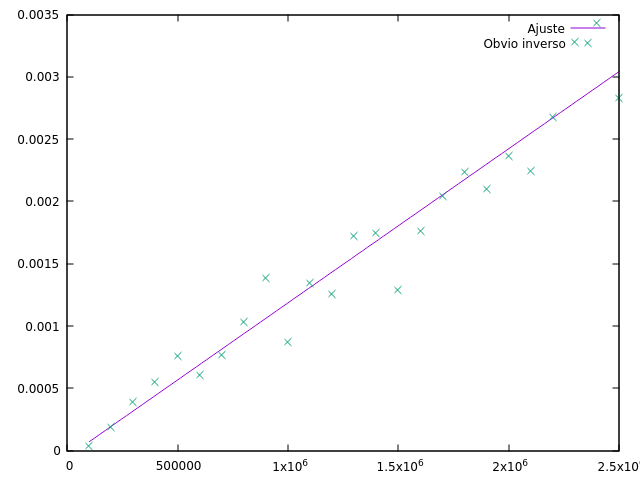
\includegraphics[width=70mm]{graficos/ajust-sol-rep}}
\end{figure}

Ahora la función de la izquierda es
$f(x)=1.31781\mbox{e}-09x-1.9522e-05$, y su ajuste tiene una RMS de
0.00021679. Mientras que la función de la derecha es
$g(x)=1.23924\mbox{e}-09-5.40427e-05$ y tiene una RMS de
0.000239843. Por tanto, estos ajustes son aproximadamente 5 veces más
precisos.
\end{document}
